\documentclass[12pt]{article}

\pagestyle{empty}
\setlength{\topmargin}{0in}
\setlength{\headheight}{0in}
\setlength{\topsep}{0in}
\setlength{\textheight}{9in}
\setlength{\oddsidemargin}{0in}
\setlength{\evensidemargin}{0in}
\setlength{\textwidth}{6.5in}

\usepackage{palatino,graphics,amsmath,amssymb,enumitem}

\newcommand{\ds}{\displaystyle}
\newcommand{\vs}[1]{\vspace{#1in}}
\renewcommand{\vss}[1]{\vspace*{#1in}}
\newcommand{\bvec}{{\mathbf b}}
\newcommand{\cvec}{{\mathbf c}}
\newcommand{\dvec}{{\mathbf d}}
\newcommand{\evec}{{\mathbf e}}
\newcommand{\fvec}{{\mathbf f}}
\newcommand{\qvec}{{\mathbf q}}
\newcommand{\uvec}{{\mathbf u}}
\newcommand{\vvec}{{\mathbf v}}
\newcommand{\wvec}{{\mathbf w}}
\newcommand{\xvec}{{\mathbf x}}
\newcommand{\yvec}{{\mathbf y}}
\newcommand{\zvec}{{\mathbf y}}
\newcommand{\zerovec}{{\mathbf 0}}
\newcommand{\real}{{\mathbb R}}
\newcommand{\twovec}[2]{\left[\begin{array}{r}#1 \\ #2
    \end{array}\right]}
\newcommand{\ctwovec}[2]{\left[\begin{array}{c}#1 \\ #2
   \end{array}\right]}
\newcommand{\threevec}[3]{\left[\begin{array}{r}#1 \\ #2 \\ #3
  \end{array}\right]}
\newcommand{\cthreevec}[3]{\left[\begin{array}{c}#1 \\ #2 \\ #3
    \end{array}\right]}
\newcommand{\fourvec}[4]{\left[\begin{array}{r}#1 \\ #2 \\ #3 \\ #4
    \end{array}\right]}
\newcommand{\cfourvec}[4]{\left[\begin{array}{c}#1 \\ #2 \\ #3 \\ #4
    \end{array}\right]}
\newcommand{\mattwo}[4]{\left[\begin{array}{rr}#1 & #2 \\ #3 & #4 \\ \end{array}\right]}
\renewcommand{\span}[1]{\text{Span}\{#1\}}
\newcommand{\bcal}{{\cal B}}
\newcommand{\ccal}{{\cal C}}
\newcommand{\scal}{{\cal S}}
\newcommand{\wcal}{{\cal W}}
\newcommand{\ecal}{{\cal E}}
\newcommand{\coords}[2]{\left\{#1\right\}_{#2}}
\newcommand{\gray}[1]{\color{gray}{#1}}
\newcommand{\lgray}[1]{\color{lightgray}{#1}}
\newcommand{\rank}{\text{rank}}
\newcommand{\col}{\text{Col}}
\newcommand{\nul}{\text{Nul}}

\begin{document}

\noindent
{\bf Mathematics 227} \\ 
{\bf Dynamical systems}

\bigskip For each of the following matrices, determine whether the
associated dynamical system is one of the six basic types we have
seen.  Sketch some trajectories to indicate the
behavior of the system below.

\begin{enumerate}
\item
  $A =
  \left[
    \begin{array}{cc}
      1.5 & -1 \\
      0.5 & 1 \\
    \end{array}
  \right].
  $

  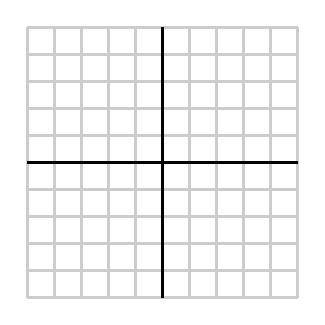
\includegraphics{empty.eps}


\item
  $A =
  \left[
    \begin{array}{cc}
      1 & -2 \\
      1 & -1 \\
    \end{array}
  \right].
  $

  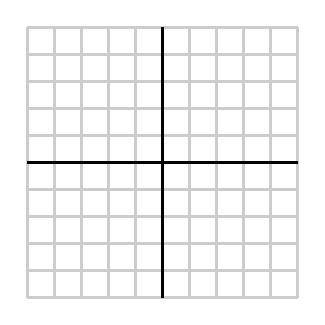
\includegraphics{empty.eps}
  
\item
  $A =
  \left[
    \begin{array}{cc}
      0.8 & -0.4 \\
      -0.2 & 1.0 \\
    \end{array}
  \right].
  $

  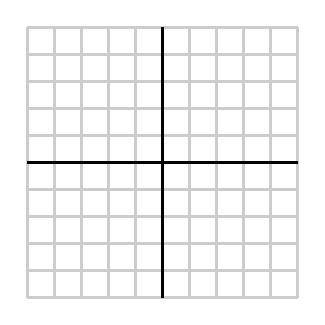
\includegraphics{empty.eps}

\item We can divide a population of female bison into three groups:
  juveniles who are less than one year old; yearlings between one and
  two years old; and adults who are older than two years.   Each year,

  \begin{itemize}
  \item 80\% of the juveniles survive to become yearlings.
  \item 90\% of the yearlings survive to become adults.
  \item 80\% of the adults survive. 
  \item 40\% of the adults give birth to a juvenile.
  \end{itemize}

  \begin{center}
    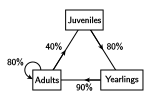
\includegraphics{eigen-3d-species.eps}
  \end{center}

  We will represent the number of juveniles, yearlings, and adults in
  year $k$ by $J_k$, $Y_k$, and $A_k$.  The state of the system in
  year $k$ will be represented by the vector
  $\xvec_k=\threevec{J_k}{Y_k}{A_k}$.

  \begin{enumerate}[label=(\alph*)]
  \item Find a matrix $B$ such that
    $
    \xvec_{k+1}=B\xvec_k
    $.

    \vs{1.5}
  \item Find the eigenvalues of $B$.  

    \vs{1.25}
    \newpage
  \item What does the size of the complex eigenvalue tell you about
    its effect on the long-term behavior of this system?

    \vs{1}
  \item An eigenvector corresponding to the real eigevalue is approximately
    $$
    \vvec = \threevec{1.000}{0.756}{2.644}.
    $$
    Make a prediction about the long-term behavior of the herd.  For
    instance, at what rate does it grow?  For every 100 adults, how
    many juveniles and how many yearlings are there?

    \vs{2}
  \item As stated, the birth rate is 40\%;  that is, 40\% of adults
    give birth to a juvenile.  Suppose this birth rate drops to 20\%.
    How does this affect the growth rate of the herd?  What does this
    mean about the long-term behavior?

    \vs{2}
  \end{enumerate}
  
  

\end{enumerate}


\end{document}
